\documentclass[12pt,a4paper]{article}

\usepackage[romanian]{babel}
\usepackage[utf8x]{inputenc}
\usepackage{amsmath}
\usepackage{graphicx}
\usepackage{gensymb}
\usepackage[colorinlistoftodos]{todonotes}
\usepackage{combelow}
\usepackage{newunicodechar}

\newunicodechar{Ș}{\cb{S}}
\newunicodechar{ș}{\cb{s}}
\newunicodechar{Ț}{\cb{T}}
\newunicodechar{ț}{\cb{t}}
\newunicodechar{Ă}{\cb{A}}
\newunicodechar{ă}{\cb{a}}
\newunicodechar{Â}{\cb{A}}
\newunicodechar{â}{\cb{a}}
\newunicodechar{Î}{\cb{I}}
\newunicodechar{î}{\cb{i}}

\title{Inside NAV}
\author{Barcan Virgil-Gheorghe}

\begin{document}
\maketitle

\begin{abstract}
Your abstract.
\end{abstract}

\section{Sistemul de operare Android}
\subsection{Despre Android}
Android este un sistem de operare dedicat dispozitivelor mobile, smartphone-uri, smartwatch-uri, precum și TV-urilor sau chiar dispozitive din interiorul automobilelor.

Sistemul de operare Android este bazat pe un kernel de Linux și a fost construit pentru a fi folosit în principal pe dispozitive touchscreen. Este cel mai folosit sistem de operare disponibil pe dispozitive mobile încă din 2013.

Sistemul a fost dezvoltat de către Android Inc., companie fondată în 2003. Dezvoltatorii au avut dorința de a ajuta la construirea de dispozitive mai inteligente, mai conștiente de locația și preferințele utilizatorilor. Sistemul de operare avea să fie un competitor pentru Symbian și Windows Mobile.

În 2005 compania Android Inc. a fost achiziționată de către Google pentru o sumă de aproximativ 50 milioane de dolari. Deși Android Inc. nu era o companie cunoscută la acel moment, intenția Google era clară pentru mulți, intrarea pe piața dispozitivelor mobile.
	
Google a oferit sistemul de operare către producători și operatori cu promisiunea de a oferi un sistem flexibil și care să poată fi actualizat. Pe lângă promisiunile făcute, Google a oferit și recomandări privind componentele hardware necesare.

La data de 5 noiembrie 2007, un consorțiu de companii precum Google, HTC, Sony, Samsung, T-Mobile, dar și producători de chipset-uri, Qualcomm și Texas Instruments, a fost lansat. Acest consorțiu, numit „Open Handset Alliance”, al cărui scop era de a dezvolta standarde deschise pentru dispozitive mobile, a lansat în aceeași zi sistemul de operare Android, ca prim produs al său.

Deși primul smartphone cu sistem de operare Android lansat a fost HTC Dream, în luna octombrie a anului 2008, au existat mai multe versiuni de prototip realizate. Una dintre aceste versiuni, numită „Sooner”, era plănuită a fi lansată ca primul telefon cu Android, însă lansarea primului iPhone a fost momentul în care a devenit clar că viitorul stătea în dispozitivele cu touchscreen. Versiunea „Sooner” era dotată cu tastatură QWERTY fizică, arătând similar unui BlackBerry.

\begin{figure}[hbtp]
\centering
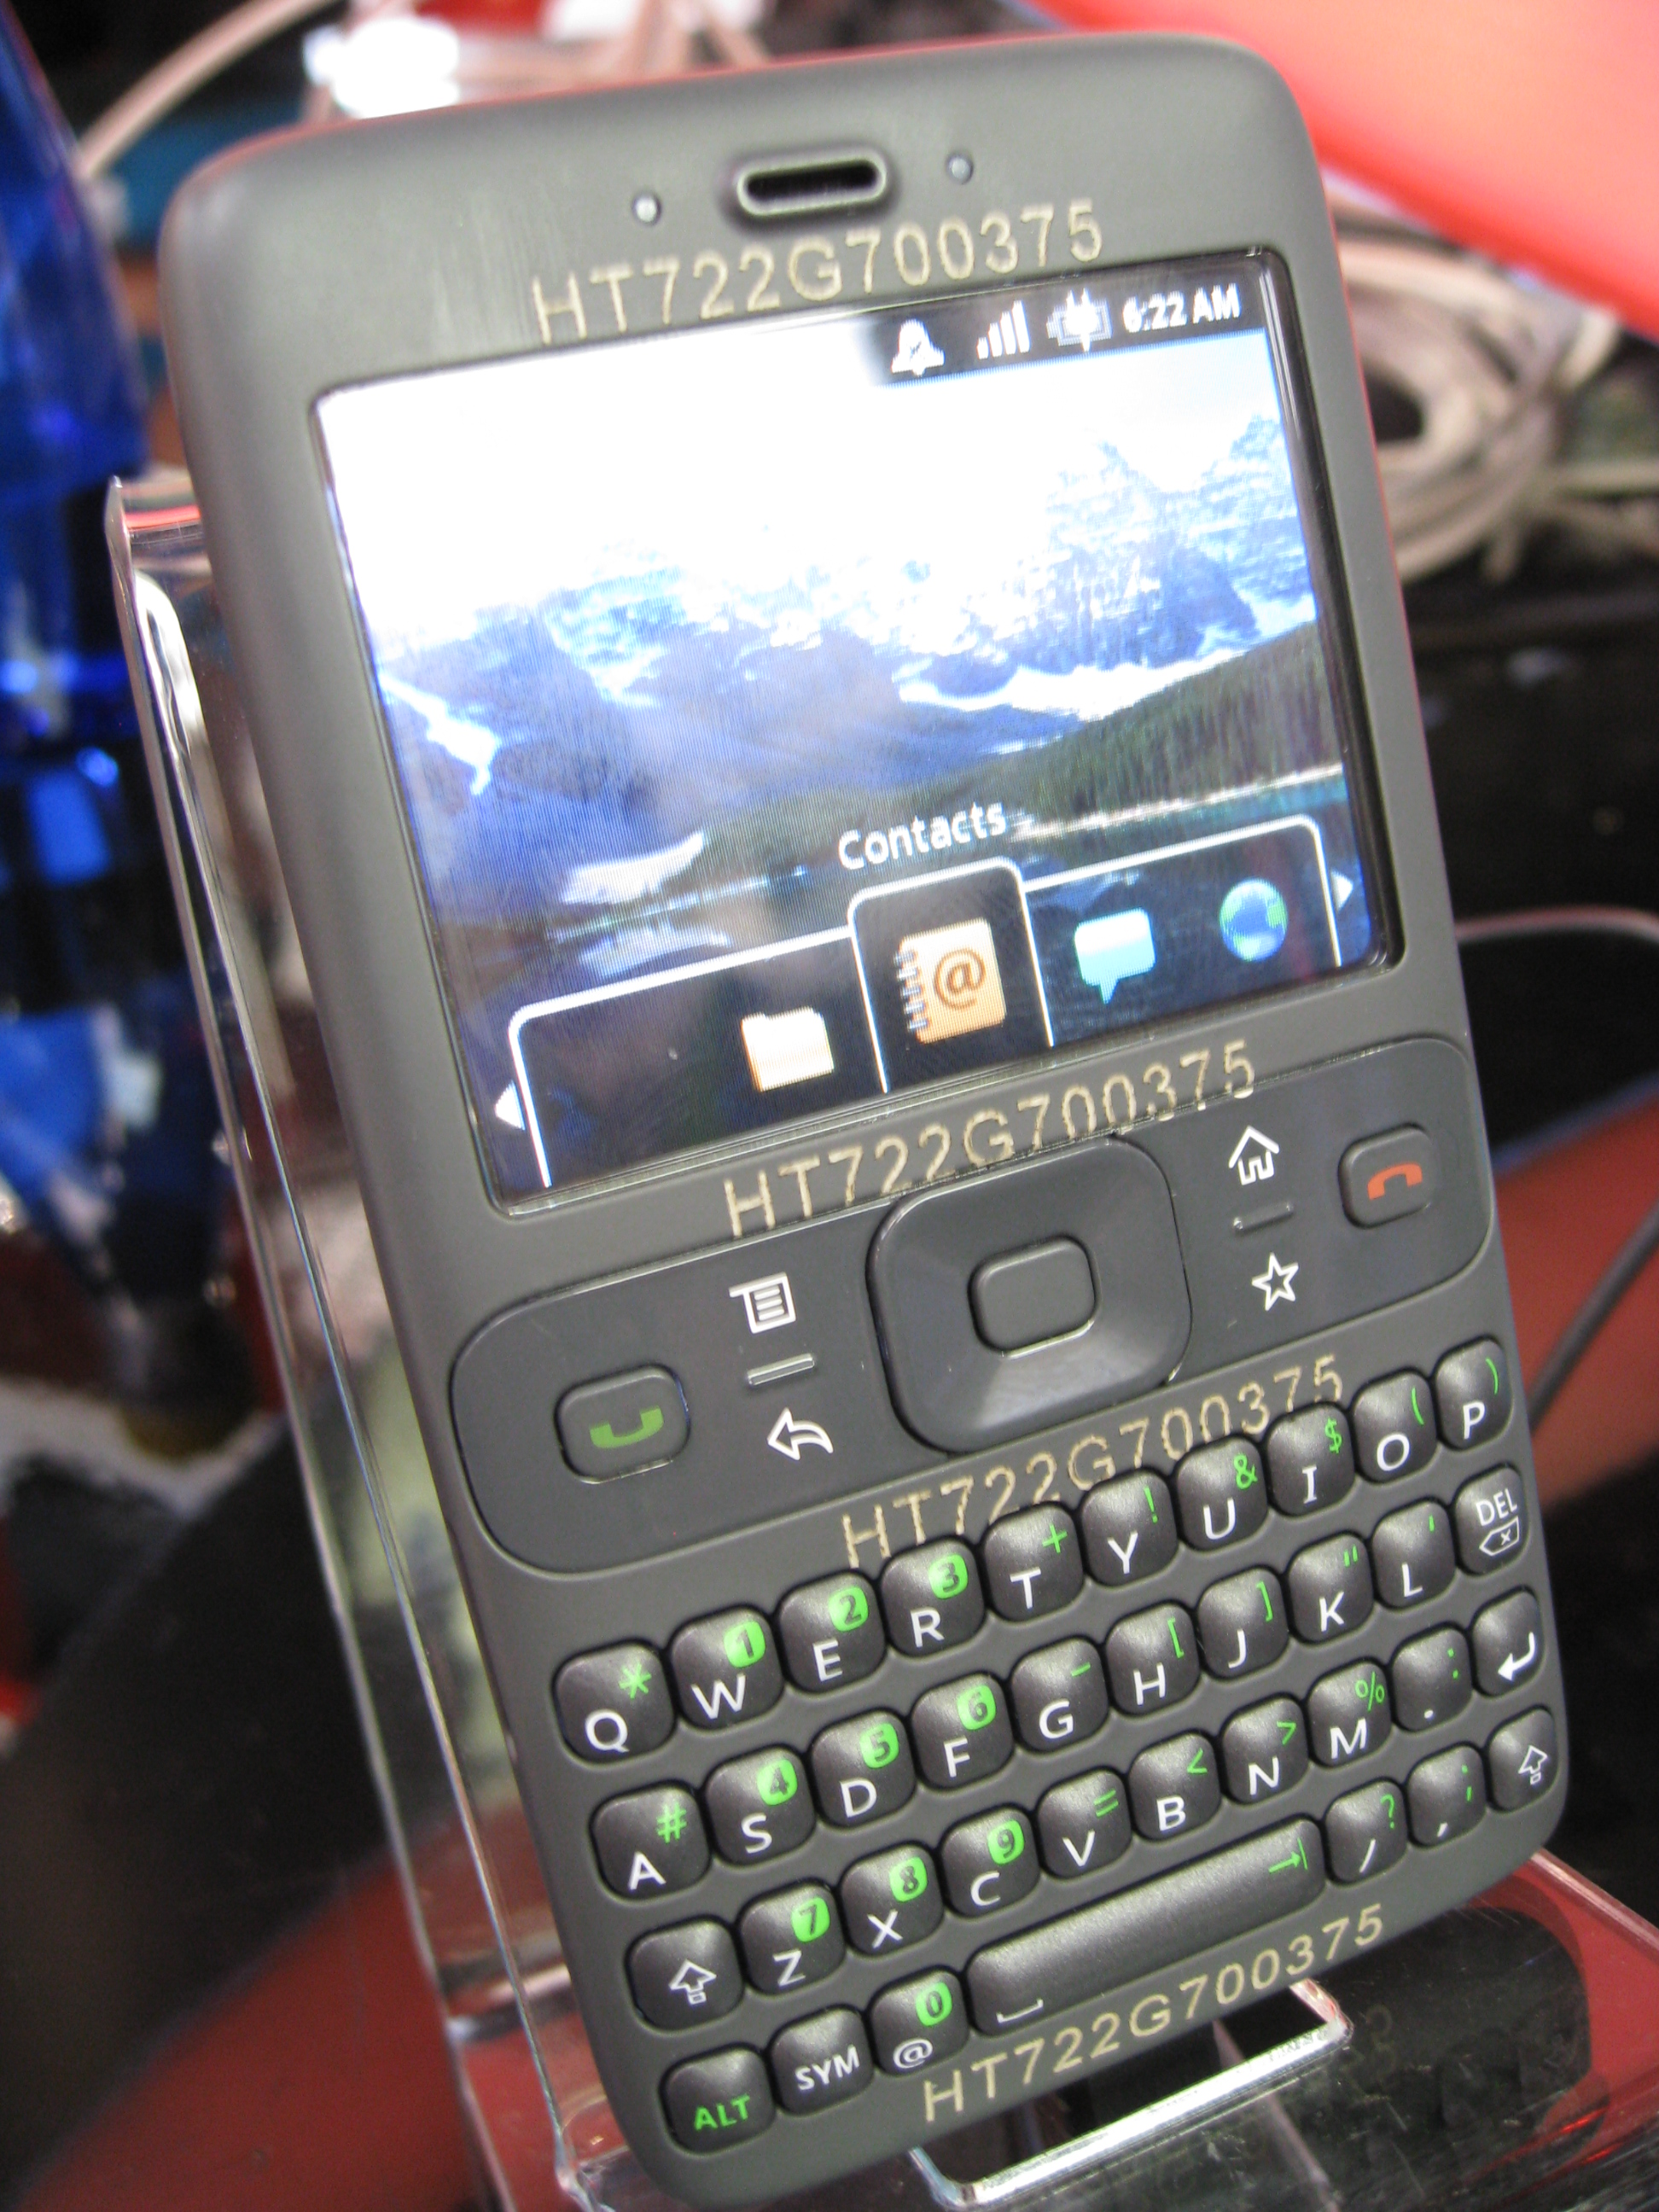
\includegraphics[scale=0.25]{figures/Android_SOONER_mobile_phone_platform_early_device.jpg}
\caption{Prototipul „Sooner”}
\end{figure}

Începând cu anul 2008 Google a adaugat noi feature-uri și a rezolvat problemele versiunilor anterioare, lansând versiuni noi ale Android.

Fiecare nouă versiune a sistemului este denumită în ordine alfabetică după un desert: „Cupcake”, „Donut”, „Eclair”, „Froyo”, „Gingerbread”, „Honeycomb”, „Ice Cream Sandwich”, „Jellybean”, „Kit Kat”, „Lolipop” și „Marshmallow”. Următoarea versiune este plănuită pentru acest an, deocamdată ea fiind denumită Android N. Google a oferit utilizatorilor posibilitatea să voteze numele.


\subsection{Versiunile Android}
\subsubsection{Android 1.0}
Prima versiune a sistemului de operare Android, denumită, deloc pompos, Android 1.0, dădea impresia de produs nefinalizat, însă lăsa să se întrevadă planurile Google pentru această platformă. Această versiune deja avea părți care, comparate cu ce era  pe piață la momentul acela, erau mult superioare. Sunt lucruri pe care acum le trecem cu vederea, dar care atunci erau noutăți, widget-urile, zonele de notificări și nu numai. 

Acestea nu doar că erau noutăți, însă și funcționau așa cum era plănuit, oferind o experiență mulțumitoare. Merită amintit și sistemul de actualizare, OTA (Over The Air), care promitea să aducă versiunile îmbunătățite într-un mod care era extrem de simplu din punctul de vedere al utilizatorului.

Prima versiune a Android includea și aplicațiile cu care suntem acum atât de obișnuiți, cum ar fi Gmail sau YouTube. Android Market Beta debuta și ea, oferind posibilitatea de a lista aplicații și jocuri, însă nu oferea posibilitatea de a plăti pentru ele.

Tot în acea perioadă Android și-a câștigat și atât de cunoscutul logo, denumit în interiorul Google „Bugdroid”.

\begin{figure}[hbtp]
\centering
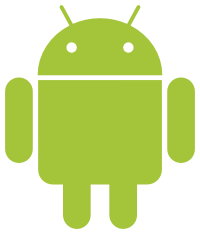
\includegraphics[scale=0.6]{figures/Android_Robot_200.png}
\caption{„Bugdroid”}
\end{figure}


\subsubsection{Android 1.5 - Cupcake}
Primul mare update al Android-ului a fost versiunea 1.5, denumită, în ceea ce avea să stabilească trendul numelor inspirate din dulciuri, „Cupcake”.

	Lansat în aprilie 2009, Cupcake a fost deschizător de drum pentru dispozitivele cu Android fără tastatură fizică. Telefoanele precedente aveau încorporate și tastaturi fizice, însă cu această versiune de sistem de operare, Google a introdus tastatura virtuală, precum și posibilitatea folosirii de tastaturi third-party. 

	Pe lângă noutățile reprezentate de tastatură, sistemul oferea și posibilitatea înregistrării de imagini folosind camera încorporată a dispozitivului, precum și un launcher îmbunătățit.

	Această nouă versiune permitea uploadul de clipuri video pe YouTube și de fotografii pe Picasa. Google a adăugat widget-uri pentru Calendar și Music. Acestea arătau evenimentele și respectiv melodia curentă. Pentru prima dată aplicațiile puteau să își adauge widget-uri proprii. O altă noutate a fost reprezentată de posibilitatea de a roti automat ecranul în funcție de orientarea telefonului, pentru o tranziție ușoară portret-landscape.


\subsubsection{Android 1.6 - Donut}
În același an al lansării Android 1.5, Google a lansat și noua versiune, 1.6, numită „Donut”.
	
	Aceasta aducea suport pentru ecrane de diferite rezoluții și densități ale pixelilor, precum și suport nativ pentru comunicarea în banda CDMA (Code Division Multiple Access). Noul sistem oferea și posibilitatea de a efectua căutări, atât în fișierele aflate pe telefon, cât și pe internet, prin așa numitul „Quick Search Box”. Tot cu această versiune a venit și posibilitatea de a vedea consumul de baterie al dispozitivului.

	Google a adus și îmbunătățiri aplicațiilor prestabilite (Gmail, Android Market). În acea perioadă, aplicațiile acestea erau considerate ca fiind parte a sistemului de operare; fiecare modificare a uneia dintre ele presupunea un nou update al softului de pe dispozitiv.
	
	Android Market a fost refăcut pentru a putea expune aplicațiile gratuite de top, precum și aplicațiile de top plătite. Acestea au fost necesare în contextul exploziei de noi aplicații de pe această platformă. Pentru prima dată au fost introduse și butoane care ofereau acces facil la setări precum Wi-Fi, Bluetooth, GPS, Sincronizare sau Luminozitate.


\subsubsection{Android 2.0, 2.0.1, 2.1 - Eclair}
Lansat în octombrie 2009, Android 2.1, denumit și „Eclair”, a adus câteva îmbunătățiri precum: posibilitatea de a căuta în toate SMS-urile și MMS-urile salvate pe telefon, viteză de tastare mărită pentru tastatura virtuală, setări de accesibilitate, calendar, dar și un API pentru VPN (Virtual Private Network). Pentru browser, Android aducea suport HTML5, precum și o interfață reîmprospătată cu posibilitatea de a salva pagini ca favorite. Tot acum au apărut double-tap- zoom și pinch-to-zoom.
	
	Ecranul de start prezenta o Google Search Bar-ul în partea superioară a ecranului. Aplicația pentru camera foto a fost și ea îmbunătățită, fiindu-i adăugate noi funcționalități precum: suport pentru pentru bliț, zoom digital, white-balance, efecte de culoare și fotografiere la nivel macro.

	Au fost introduse și ecranele de fundal animate, butoanele pe ecran (oferind posibilitatea de a accepta/respinge apeluri, ceea ce a dus la dispariția nevoii de butoane fizice). Tot în versiunea Eclair a fost introdusă și posibilitatea de a folosi Google Maps pentru navigație, aceasta oferind indicații pas-cu-pas, dar și informații legate de trafic, caracteristici similare serviciilor de navigație din automobile, cu diferența că cele oferite de Google erau gratuite.

	O altă funcționalitate care acum este extrem de utilizată și a fost adăugată înca din versiunea Eclair este cea de Speech-to-Text, care permitea introducerea de text dictând telefonului. Acum folosim cu toții funcții precum „Ok Google” și efectuăm căutări folosind aceste funcții.
	

\subsubsection{Android 2.2 - Froyo}
Poate cea mai importantă noutate a acestei versiuni a fost aceea a introducerii mașinii virtuale Dalvik, care oferea Just-in-time Compiling, oferind îmbunătățiri masive ale vitezei Android-ului.

	Cu această versiune a fost oferită și posibilitatea de a instala sau muta aplicațiile pe cardul de memorie pentru a elibera memoria internă a telefonului. Altă noutate a fost reprezentată de hotspot-ul Wi-Fi, care permitea telefonului să ofere Wi-Fi altor dispozitive.

	Browser-ul a cunoscut și el îmbunătățiri ale vitezei prin schimbarea motorului de JavaScript la cel folosit de Chrome, V8. Această schimbare a adus viteze de 2 până la 5 ori mai mari ale browser-ului. Tot acum s-a introdus și suportul pentru Flash, permițând o experiență similară celei de pe un browser desktop.

	Au fost adăugate aplicații noi, cum ar fi Google Goggles, care permitea efectuarea de căutări folosind camera telefonului.


\subsubsection{Android 2.3, 2.3.3 - Gingerbread}
Cu această nouă versiune a Android a apărut și ceea ce avea să devină un nou obicei al Google, acela de a lansa un telefon sub marcă proprie cu fiecare versiune nouă a soft-ului. Aceasă linie de telefoane se va numi Nexus și va fi construită cu producători diferiți la fiecare nouă iterație, ea oferind un Android „curat”, neîncărcat de aplicații oferite de producători sau operatori. Primul telefon din gama Nexus a fost Nexus S, oferit de către Google în parteneriat cu Samsung.

	Sistemul de operare a adus suport pentru NFC (Near Field Communication), pentru ecrane cu rezoluții mari, pentru telefonie via internet (VoIP), dar și îmbunătățiri ale interfeței vizuale.

	Noul garbage collector concurent a adus un spor de viteză. A fost mărită și viteza de distribuție a evenimentelor în sistem. Tot cu această versiune s-a adăugat și suport nativ pentru mai mulți senzori (cum ar fi giroscopul și barometrul), suport pentru multiple camere video, dar și posibilitatea efectuării de apeluri video.

	Pentru dezvoltatori a fost îmbunătățit suportul pentru scrierea de cod nativ și s-au introdus API-urile pentru jocuri.


\subsubsection{Android 3.0 - Honeycomb}
Această nouă versiune a fost lansată cu scopul de a îmbunătăți experiența de utilizare a sistemului pe tablete. Pe lângă îmbunătățirile aduse la nivelul interfeței grafice, au fost aduse și îmbunătățiri la nivelul suportului pentru procesoare multi-core.

	A fost introdus și API-ul pentru utilizarea Fragmentelor, care permiteau dezvoltatorilor de aplicații sa folosească suprafața mai mare a ecranului unei tablete pentru a afișa mai multe părți ale aplicației. Folosirea Fragmentelor permitea separarea aplicațiilor pentru telefoane de cele pentru tablete într-un mod foarte simplu: dacă exista suficient spațiu, se afișau mai multe fragmente ale aplicației, altfel se afișa doar unul și utilizatorul trebuia să navigheze între acestea.

	A fost introdus și conceptul de Action Bar, adică acel spațiu din partea superioară a unei aplicații similar unui meniu dintr-o aplicație desktop. Acesta îți permitea să navighezi înapoi, să vezi unde te afli în aplicație, să intri în setări sau în alte zone considerate ca fiind cele mai utile de către dezvoltator.

	Browserul a primit suport pentru tab-uri, similar browserului de pe desktop. A fost introdusă și posibilitatea sincronizării browserului de pe telefon cu cel de pe desktop, pentru a oferi o experiență integrată.

	Această versiune a sistemului de operare nu a fost oferită ca open-source, iar toate dispozitivele care o foloseau au fost actualizate la versiunea superioară, Ice Cream Sandwich.


\subsubsection{Android 4.0 - Ice Creak Sandwich}
Această versiune oferea o experiență unificată smartphone-tabletă, ea înlocuind complet versiunea Honeycomb și aducând noutățile ei și pe smartphone-uri.

	A fost îmbunătățit multitaskingul, notificările au devenit mai bogate, ecranul de start au fost și el modificat, acum putându-se adăuga foldere pe acesta, pentru a se reduce consumul de spațiu. S-a adăugat un sistem de management al consumului de date prin care se puteau urmări consumul fiecărei aplicații și impune limite de utilizare.

	Multitaskingul a devenit acum mai vizibil pentru utlizatorul final, acesta putând acum să selecteze aplicația pe care să o redeschidă. Utilizatorul poate vedea o listă de aplicații pe care le-a folosit în ultima perioadă, apoi poate selecta aplicația pe care să o readucă în prim-plan.

	În partea de jos a ecranului au apărut aplicațiile favorite, într-un aranjament similar celui de pe iPhone. Au mai fost adăugate ecrane noi de blocare, precum și de acceptare/respingere apeluri. Gesturile încep să devină parte esențială a experienței de utilizare a smartphone-ului, ele putând fi folosite pentru a șterge notificări, pentru a schimba tab-urile în browser, dar și pentru a respinge/accepta apeluri, așa cum am spus și mai sus.

	Una din inovațiile aduse a fost Android Beam. Acest sistem permitea transferul de date între dispozitive care dispuneau de NFC. Acest transfer se făcea cu viteze mai mari decât ale Bluetooth-ului, de exemplu. Modalitatea de utilizare era extrem de facilă din perspectiva utilizatorului. Acesta trebuia doar să apropie cele două dispozitive și să apese „Trimitere”.

	Undeva între versiunile Ice Cream Sandwich și Jelly Bean, Android Market a devenit Google Play store. Împreună cu redenumirea acestei aplicații au fost modificate și celelalte aplicații: Play Music, Play Books, Play Movies.


\subsubsection{Android 4.1, 4.2, 4.3 - Jelly Bean}
Această iterație a Android a adus noi îmbunătățiri la capitolul viteză prin introducerea „Project Butter”, care implementa Vsync și triple-buffering. Notificările au fost și ele modificate, acum fiind posibil ca utilizatorul să le poată mări. Notificările puteau conține până la 8 linii de text și chiar butoane la baza lor. Aceste butoane puteau fi folosite pentru a lua acțiuni în funcție de notificare: de exemplu, dacă se primea un SMS, se putea apăsa un buton care să pornească aplicația prestabilită de mesagerie gata de a oferi răspuns mesajului.

	În Android Jelly Bean a fost lansat și Google Now, asistentul virtual al Google. Acesta oferă informații legate de vremea din locația curentă, precum și despre timpii necesari pentru a ajunge între diferite locații. Această aplicație este acum parte integrată a experienței de utilizare a Android.

	Printre noutăți se numără și posiblitatea de a avea mai multe conturi pe același dispozitiv. Au fost introduse și widget-uri direct în ecranul de blocare, care permitea utilizatorilor să interacționeze cu aplicațiile fără să deblocheze telefonul. Tot acum s-a adăugat și suportul pentru ecrane externe, eventual via Miracast (Wi-Fi Display).

	Alte îmbunătățiri sunt date de adăugarea HDR (High Dynamic Range), a Bluetooth Low Energy și a OpenGL ES3.0, care aducea sporuri de performanță la nivel grafic.


\subsubsection{Android 4.4 - KitKat}
Poate cea mai importantă funcționalitate adăugată cu această versiune este cea a interacțiunii cu telefonul prin comenzi vocale. Faimosul „Ok, Google” a fost oferit începând cu această versiune. Tot acum s-au făcut eforturi pentru ca Android să poată rula mai bine pe dispozitive mai slabe din punct de vedere hardware. Acum Android putea rula chiar și pe 512 MB de RAM.

	Aplicațiile pot fi lansate cu adevărat în modul ecran complet începând cu KitKat. Până la această versiune aplicațiile ocupau tot ecranul, mai puțin status bar-ul. Se îmbunătățește securitatea tranzacțiilor realizate prin NFC prin implementarea  HCE (Host Card Emulation).

	Google Drive devine o aplicație de legătură către aplicațiile office ale Google. Hangouts suporta SMS-uri, de aceea acum se elimină aplicația de mesaje. Atunci când se scrie un număr nou pentru a se efectua un apel, Android caută în punctele de interes din apropiere pentru a găsi informații suplimentare despre destinatar.

	S-a adăugat posibilitatea printării oricărui conținut folosind o rețea Wi-Fi sau servicii cloud de tipul Google Cloud Print. S-a adăugat și un nou sistem de acces la stocare, care a permis dezvoltatorilor precum Box sau Dropbox să integreze serviciile lor direct cu memoria telefonului, oferind acces facil la documente din locații diferite.

	Au fost imbunătățiți și senzorii, prin reducerea consumului lor de baterie. Android nu  mai trimite notificările imediat cum senzorii observă modificările, ci le stochează până are suficiente.  Acest mod de lucru este ideal pentru aplicațiile care au nevoie de acces permanent la datele senzorilor, cum ar fi aplicațiile de fitness. Legat de aplicații de fitness, acum au fost introduși și senzorii de detectare a pașilor și de numărare a pașilor. Acești doi senzori folosesc date de la senzorii disponibili pe dispozitiv și, aplicând algoritmi de fuziune a datelor primite, deosebesc pașii efectuați de utilizator.


\subsubsection{Android 5.0, 5.1 - Lollipop}
Android Lollipop a fost versiunea în care a apărut noul stil vizual propus de Google, „Material Design”. Acest ghid despre cum trebuie să arate interfața vizuală a aplicației a fost un mare pas către unificarea experienței de utilizare a aplicațiilor de pe această platformă.
	
	Material Design este un set de reguli de design inspirat din modul în care arată hârtia în diferite combinații de lumini și umbre.
Componentele grafice din aplicații erau acum reprezentate într-un mod minimalist, ca și cum ar fi niște colaje de hârtie. Google nu a adus doar recomandările legate de cum trebuie să arate componentele grafice, ci și un întreg set de instrumente noi care să ajute dezvoltatorii. Au fost introduse animații la trecerea dintre activități, la apăsarea butoanelor, la apăsarea pe câmpuri de text și nu numai. A fost introdus și un nou thread pe care să se facă toate animațiile, pentru a se garanta că acestea sunt cât mai fluente.
	
	Android 5.0 a adus și îmbunătățiri de performanță prin adăugarea ART runtime în locul Dalvik. Acum există suport pentru procesoare cu arhitectura pe 64 de biți. S-a adăugat suport pentru OpenGL ES 3.1, care a dus la jocuri mai bogate grafic și mai captivante.
	
	Tot începând cu această versiune Android și-a făcut apariția și în zona TV, prin lansarea Android TV. Acest sistem rula pe televizoare, oferind funcționalități similare celor de pe smartphone-uri, jocuri, aplicații, dar și experiența unui TV normal. Dar Android nu s-a oprit la zona TV, el apărând și în zona auto, prin Android Auto, un sistem care permite smartphone-ului să se conecteze la mașină și să primească date de la senzorii acesteia. Smartphone-ul are acces și la ecranul dispozitivului, pe care afișează o interfață simplificată, pentru a nu distrage șoferul.

	În această iterație a fost adăugat și suportul pentru HD voice, care face ca apelurile să fie mai clare. Suportul pentru dual-SIM a fost introdus tot acum.

	
\subsubsection{Android 6.0 - Marshmallow}
Android Marshmallow a introdus un nou sistem de permisiuni pentru aplicații. Acest nou model presupunea ca aplicația să ceară drepturi de la utilizator nu la instalare, ci atunci când îi era necesar. Prin acest nou set de reguli se dorea ca utilizatorii să știe mai clar ce acceptă, deoarece înainte utilizatorii nu erau neapărat atenți la ce acceptau, și puteau exista aplicații care să poată avea acces la mai multe date decât le era necesar. Existau aplicații de genul „Lanternă” care aveau acces la contacte, locație, microfon și cameră. Genul acesta de permisiuni sunt în mod clar un pericol la intimitatea utilizatorilor, iar cu Android 6.0 Google a încercat să îl limiteze.

	O altă componentă a sistemului unde cei de la Google au adus îmbunătățiri este cea a consumului de baterie. Prin adăugarea „Doze” și a „App Standby”, aplicațiile consumă acum mai puțină baterie. Doze pune sistemul într-o stare de sleep atunci când acesta nu este conectat la o sursă de energie. În mod regulat sistemul repornește pentru scurte perioade de timp pentru a efectua sarcinile care sunt în așteptare. App Standby permite sistemului să determine ce aplicație este idle atunci când utilizatorul nu o folosește. Sistemul oprește accesul la rețele pentru astfel de aplicații, dar și oprește eventualele job-uri ale acestora.

	În Marshmallow s-a adăugat și Now On Tap, un asistent virtual care permite să afli informații fără să părăsești aplicația curentă. Este util atunci când vrei să afli ce reprezintă ceva din aplicația curentă. Android recunoaște cuvinte sau imagini reprezentative și îți afișează rezultatele unei căutări după acestea. Să presupunem că folosești o aplicație de redare audio și vrei să afli cine este cântărețul principal. Pur și simplu spui: „Ok, Google, cine este liderul trupei?”. Now On Tap va ști la ce trupă te referi deoarece știe ce asculți, aplicația ta curentă fiind redare audio.


\subsubsection{Android N}
O nouă versiune a Android este în dezvoltare acum, aceasta având numele de cod „Android N”. Un nume care să urmeze linia numelor inspirate din produse dulci este în curs de a fi ales, Google oferind utilizatorilor posibilitatea să recomande și să voteze numele.
	
	Versiunea Android N este acum în developer preview, ceea ce înseamnă că există oameni care deja au această versiune pe device. Aceast Android promite îmbunătățiri în 3 zone cheie: performanță, productivitate și securitate. Noul JIT compiler va duce la instalări mai rapide ale aplicațiilor, plus spațiu mai mic ocupat de către acestea. Noua bibliotecă de randare 3D, numită „Vulkan”, promite performanțe sporite, în special pentru zona jocurilor. 
	
	Modificările nu se vor opri aici, ci vor include, pentru prima dată în Android, suport pentru mai multe ferestre, similar modului în care Windows 8 permitea deschiderea în paralel a mai multor aplicații. Android Instant Apps va permite testarea unor aplicații fără ca acestea să fie instalate efectiv pe dispozitiv.	
	
	Se va aduce și un Doze îmbunătățit, plus noi schimbări în ceea ce privește permisiunile aplicațiilor. Se vor aduce îmbunătățiri și în zona accesibilitații, prin implementarea „Screen Zoom”.
	
	

\subsection{Senzorii disponibili pe platforma Android}
Majoritatea dispozitivelor care rulează Android au încorporați diverși senzori. Aceștia sunt folosiți în diferite contexte în timpul folosirii dispozitivului. Scopul senzorilor este să urmărească eventuale schimbări astfel încât sistemul să răspundă în cel mai bun mod cu putință.

	Deși poate nu este evident, întreaga experiență de utilizare a telefonului/tabletei este dependentă de senzori. Faptul că ecranul se închide atunci când apropiem telefonul pentru a vorbi, faptul că putem să ne măsurăm distanțele parcurse, caloriile consumate, bătăile inimii, faptul că putem să folosim telefonul ca sistem de navigație, toate acestea se datorează folosirii senzorilor.
	
	Android împarte senzorii în mai multe categorii, deși tratarea lor se face într-un mod aproape unitar: 
\begin{itemize}
\item Senzori de mișcare,
\item Senzori de mediu,
\item Senzori de poziție,
\item Senzori de locație.
\end{itemize}

	Încă un mod în care Android împarte senzorii este acela că senzorii pot fi \textbf{hardware} sau \textbf{software}. Senzorii hardware sunt efectiv piese fizice capabile să măsoare diferite schimbări. Ei notifică sistemul de eventuale schimbări. Senzorii software sunt senzori care combină datele de la mai mulți senzori pentru a obține un nou set de măsurători. Scopul lor este de a scuti dezvoltatorii să rescrie aceleași rutine de fiecare dată când au nevoie de date care nu sunt deja oferite. Rutinele acestea sunt algoritmi complecși, nu neapărat ușor de scris.\\
	
\subsubsection{Sistemul de coordonate al senzorilor}
În general Android folosește un sistem de coordonate standard, cu 3 axe. Valorile venite de la senzori reprezintă schimbările pe aceste trei axe.

Sistemul de coordonate este definit în raport cu ecranul dispozitivului (ținut în pozitie verticală), astfel: axa $X$ este orizontală și orientată către dreapta, axa $Y$ este verticală si orientată către partea superioară a dispozitivului, iar axa $Z$ este axa care „iese” din centrul ecranului.

\begin{figure}[hbtp]
\centering
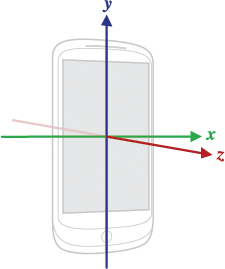
\includegraphics[scale=0.8]{figures/axis_device.png}
\caption{Sistemul de coordonate}
\end{figure}

Ce este extrem de important de rețiunt este că axele nu se schimbă atunci când dispozitivul este mișcat. Sistemul de axe este definit în raport cu orientarea normală a ecranului, care este, pentru smartphone-uri, portret, însă nu este obligatoriu să fie așa pentru orice dispozitiv. De exemplu tabletele sunt cel mai adesea orientate landscape.\\

\subsubsection{Senzori de mișcare}
Acești senzori oferă posibilitatea monitorizării mișcării dispozitivului, de exemplu rotație, scuturare, înclinare sau legănare. Doi dintre acești senzori sunt mereu senzori fizici: \textbf{accelerometrul} și \textbf{giroscopul}. Ceilalți trei senzori pot fi atât hardware, cât și software: \textbf{senzorul de gravitație}, \textbf{senzorul de accelerație liniară} și \textbf{senzorul vectorului de rotație}. Recent au fost adăugați și senzori de \textbf{detectat}, respectiv \textbf{numărat pași}.

	\textbf{Accelerometrul} determină accelerația aplicată dispozitivului prin măsurarea forțelor aplicate senzorului în sine. Totuși, în aceste măsurători intră mereu în calcul gravitația. Astfel, chiar dacă telefonul stă orizontal nemișcat, accelerometrul înregistrează o magnitudine de $g = 9,81$ $m/s^{2}$.

	\textbf{Senzorul de gravitație} oferă un vector 3-dimensional care indică direcția și magnitudinea gravitației.

	\textbf{Senzorul de accelerație liniară} oferă un vector 3-dimensional care indică accelerația pe fiecare axă, excluând gravitația.

	Putem formaliza relația dintre accelerații astfel:
	$A_{liniara} = A - g$.\\

	\textbf{Giroscopul} măsoară viteza angulară în raport cu axele $X$, $Y$, $Z$. Viteza angulară este măsurată în $rad/sec$.\\

	\textbf{Senzorul vectorului de rotație} reprezintă orientarea dispozitivului ca fiind combinația dintre o axă și un unghi în care acesta este rotit în jurul uneia dintre axele $X$, $Y$, $Z$ cu un unghi $\theta$. Cele trei componente ale vectorului de rotație sunt: $(x \sin{\theta}, y \sin{\theta}, z \sin{\theta})$. 
	
	Comparativ cu ceilalți senzori de mișcare, acest senzor are valorile exprimate într-un alt sistem de coordonate, unul „global”.
	Acest sistem are următoarele caracteristici:
	\begin{itemize}
	\item $X$ este definit ca fiind tangent la pământ în locația curentă și orientat către Est,
	\item $Y$ este definit ca fiind tangent la pământ în locația curentă și orientat către Polul Nord Magnetic,
	\item $Z$ este definit ca fiind perpendicular la planul definit de $X$ și $Y$ si orientat către cer.
	\end{itemize}

\begin{figure}[hbtp]
\centering
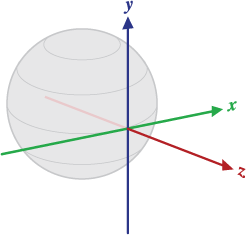
\includegraphics[scale=0.8]{figures/axis_globe.png}
\caption{Sistemul de coordonate utilizat de senzorul vector de rotație}
\end{figure}


\subsubsection{Senzori de mediu}
Acești senzori permit monitorizarea unor valori precum \textbf{umiditatea}, \textbf{intensitatea luminoasă}, \textbf{presiunea atmosferică} sau \textbf{temperatura mediului} din apropierea dispozitivului. Toți senzorii menționați sunt hardware.

Senzorii de intensitate luminoasă, presiune și temperatură sunt unii dintre cei mai simplu de utilizat. Ei oferă valori cu următoarele unități de măsură: $lx$ (lux) pentru intensitatea luminoasă, $mbar$ (milibar) pentru presiunea atmosferică, respectiv $\celsius$ (grade Celsius) pentru temperatură.

\subsubsection{Senzori de poziție}
Acești senzori permit monitorizarea poziției dispozitivului într-un cadru de referință global, prin urmărirea schimbărilor de \textbf{câmp magnetic} sau a \textbf{orientării}.



\subsubsection{Senzori de locație}
Acești senori primesc date despre locația GPS curentă a dispozitivului.



Deși acești senzori sunt recunoscuți de către Android, nu este obligatoriu ca toți să fie prezenți.





\end{document}